\chapter{Toward real-time, kinetic studies of promoter escape by RNAP}
\label{chpt:towards_promoter-escape_movie}

RNAP plays a pivotal role in gene regulation by catalyzing the transcription reaction, which results in the production of \ac{mRNA}, please refer to Sections~\ref{sec:rnap_intro} and \ref{sec:RNAP_cycle} for a detailed discussion. 
Briefly, \ac{mRNA} serves as an important intermediary for protein synthesis, and ultimately influences the phenotype of the cell.
As described previously, promoter escape is the the rate-limiting step in the process of transcription initiation~\cite{murakami_structural_2002}. 
Thus promoter escape acts as an important checkpoint in gene regulation.

Moreover, bacterial \ac{RNAP} studies hold significant relevance in the broader scientific and medical community. 
Understanding the dynamics of \ac{RNAP} and, in particular, unraveling the intricate details of promoter escape can provide valuable insights for the development of antibiotics. 
%as well as \enquote{general} science.
%That is, scientific studies for the sake of expanding our collective knowledge.
By better understanding the intricacies of promoter escape, we can expand the phase space for drug discovery, identifying specific time points during which we can intervene and disrupt short-lived conformations critical for the bacterial enzyme's function.

The ability to investigate these dynamic processes at the single-molecule level, in real-time, is an exciting and lofty goal. 
Current methods lack the temporal resolution needed to observe non-equilibrium structural changes as a function of time, especially in the context of processes like protein folding or rapid structural conformational changes. 
The development of a \ac{HT-smFRET} platform for the purpose of time resolved, atomically accurate \enquote{movies} of such dynamic molecular processes, is a groundbreaking, albeit extremely challenging, endeavor.

In my thesis work, I have laid the foundation for such a platform, and I utilize the study of the \ac{RNAP} promoter escape mechanism as an illustrative example of this novel method which has broader application in the field of structural biology.
The real-time, single-molecule approach being developed in this research represents a pioneering step towards achieving this goal.

%%%%%%%%%%%%%%%%%%%%%%%%%%%%%%%%%%%%%%%%%%%%%%%%%%%%%%%%%%%%%%%%%%%%%%%%%%%%%%%%%%%
\section{Experimental design for kinetic studies of promoter escape}
\label{sec:promoter_escape_exp}

The experimental approach for conducting freely-diffusing \ac{HT-smFRET} studies of \ac{RNAP} promoter escape involves several key steps:

\begin{enumerate}
    \item Labeling strategy for \ac{HT-smFRET} studies of \ac{RNAP}
    \item Creation of a distance network for molecular simulations using FRET-derived distances
    \item Control experiments on the single-spot \ac{ALEX} setup
    \item Transition to 32-spot \ac{HT-smFRET} platform for real-time, kinetic studies
\end{enumerate}

Through this series of biophysical experiments, this work establishes the foundational components of a \ac{HT-smFRET} methodology, enabling the investigation of the dynamic mechanisms involved in \ac{RNAP} promoter escape. 
The ultimate objective is to advance our understanding of \enquote{basic} science using this novel biophysical approach.

\section{Generating a $\sigma^{70}$ mutant library}
\label{sec:sigma70_library_exp}

In order to use \ac{smFRET} to study any biological system, it is necessary to label the molecules of interested with fluorophores.
As fluorescent dyes are sufficiently small and bright, they more closely meet the condition of a point dipole approximation, where the size of the fluorophore is much smaller than $R$, as discussed in Section~\ref{sec:FRET_theory}.
Thus, in comparison to fluorescent proteins or quantum dots, fluorescent dyes remain the ideal choice for labeling in the context of \ac{smFRET}.

To perform \ac{smFRET} studies on promoter escape in \ac{E. coli} \ac{RNAP}, we developed a strategy for generating singly-labeled $\sigma^{70}$ constructs. 
We targeted $\sigma^{70}$, as the removal of the $\sigma_{3.2}$ loop during promoter escape has yet to be observed. 
To this end, I created a plasmid library, which would subsequently serve as the foundation for generating a protein library of single-cysteine $\sigma^{70}$ mutants. 
The ultimate aim being to utilize this protein library to construct a comprehensive distance network, a concept that will be explored in greater detail in Section~\ref{sec:distance_network_exp}.

To facilitate labeling using cysteine chemistry, we initiated the process by eliminating all native cysteine residues within the \ac{wt-rpoD} gene that codes for the $\sigma^{70}$ factor. 
This was achieved using standard \ac{PCR} techniques for point mutagenesis, where every cysteine was systematically mutated into a serine. 
This mutation is commonly referred to as a \enquote{Cys to Ser mutation.} 
These constructs will be referred to throughout as \enquote{cystiene-less} mutants, denoted as rpoD(-C).
By removing all native cysteines, we could subsequently introduce a single cysteine at locations of interest, where a dye could be conjugated. 
Thus we created a series of $\sigma^{70}$ factors labeled at different amino acid locations with a single donor dye via cysteine chemistry.

\subsection{Creation of donor-labeled library of $\sigma^{70}$ constructs}
\label{sec:plasmid_lib_exp}

\begin{figure}
    \centering
    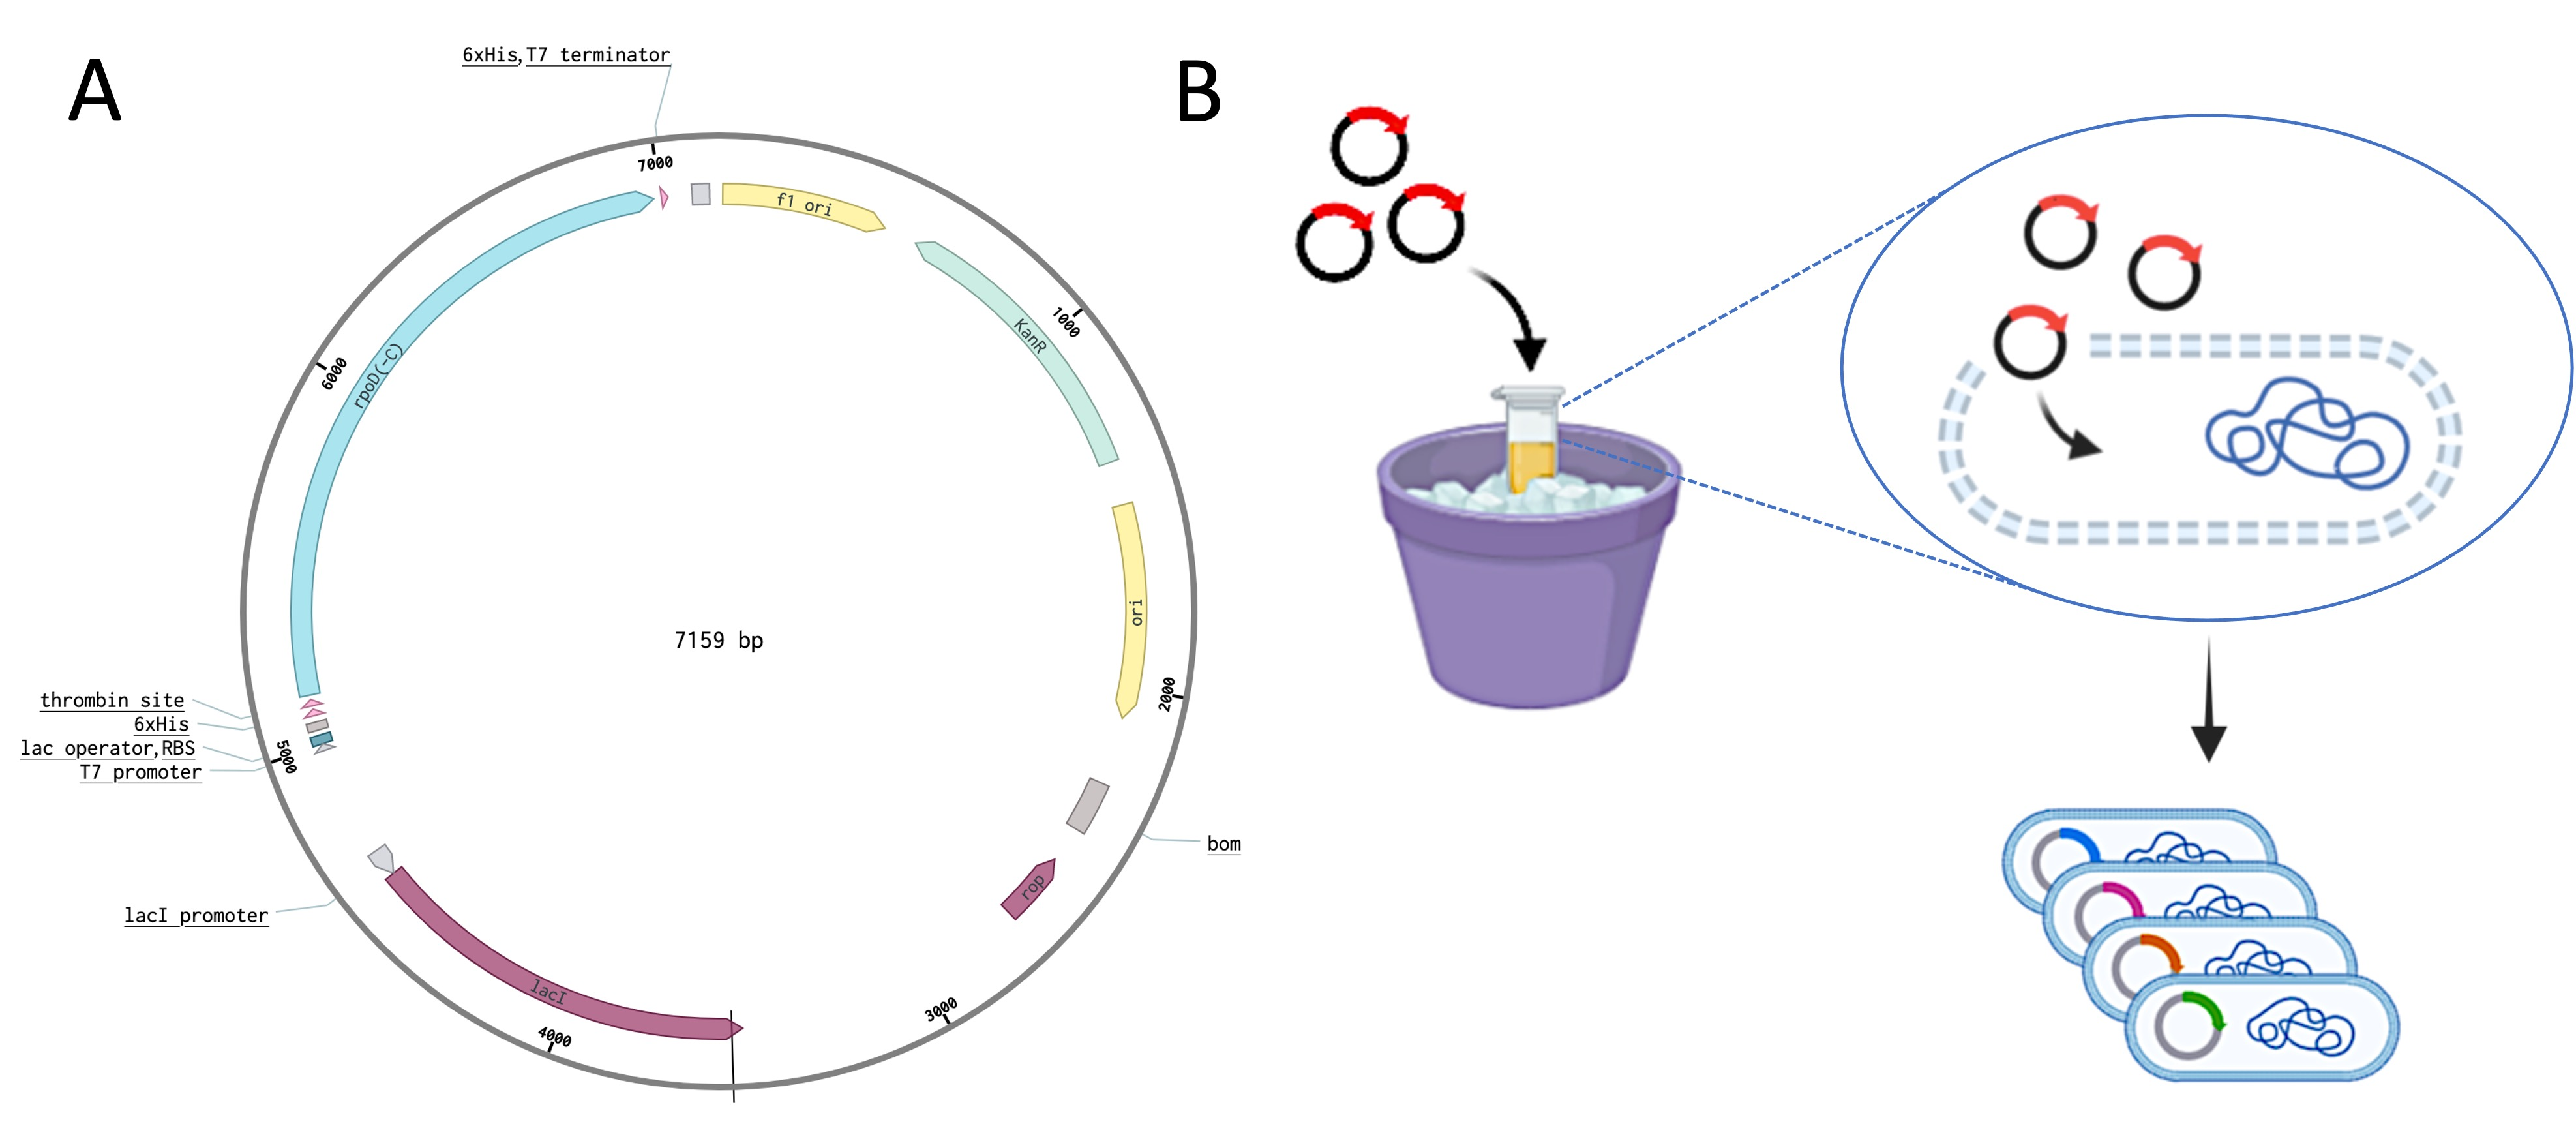
\includegraphics[width=\textwidth]{chapters/figures/plasmid_library.jpg}
    \caption{\label{fig:plasmid_library} 
    Generation of a plasmid library.
    A) pET28(+) plasmid map containing the rpoD(-C) gene, referred to throughout as pET28(+)-rpoD(-C).
    Note that the pET28(+) plasmid contains a kanamycin resistance gene (KanR, cyan arrow) for selection after transformation.
    The pET28(+) plasmid also contains flanking T7 promoter and terminator sequences along with His6x tags for purification after protein over-expression (performed by Dr. Sergei Borukhov, not shown).
    B) The pET28(+)-rpoD(+C) plasmids (black circle with red insert) were transformed into Ca$^{2+}$-competent TOP-10 cells via heat shock (indicated by the ice bucket). 
    This step reintroduced a cysteine at various locations on the $\sigma_{3.2}$ loop, thereby generating the plasmid library. 
    Different colored inserts signify unique rpoD(+C) constructs within the library.
    }
\end{figure}

The pET28(+) plasmid, containing a kanamycin resistance gene (KanR), was transformed with the \ac{wt-rpoD} insert into Ca$^{2+}$-competent TOP-10 cells.
Subsequently, cysteines were iteratively removed through \ac{PCR}, resulting in the pET28(+) plasmid with rpoD(-C) inserted between positions 5140 and 6981. 
Refer to Figure~\ref{fig:plasmid_library}A for the plasmid map of pET28(+) with the rpoD(-C) insert, further denoted as pET28(+)-rpoD(-C).

The plasmid library was established by introducing a single cysteine at various locations within and around the $\sigma_{3.2}$ and $\sigma_{3/4}$ regions. 
Single-cysteine inserts, denoted as rpoD(+C), were generated using standard \ac{PCR} techniques with pET28(+)-rpoD(-C) as the template DNA.
The product of these reactions was the single-cysteine containing plasmid, denoted here as pET28(+)-rpoD(+C).

In this notation, pET28(+)-rpoD(+C) serves as a generalized representation indicating the presence of a cysteine mutation. 
For instance, pET28(+)-rpoD(I511C) signifies the mutation of isoleucine (I) at the 511 amino acid position to cysteine (C). 
Figure~\ref{fig:plasmid_library}B provides a visual representation of the transformation process for the pET28(+)-rpoD(+C) plasmids into Ca$^{2+}$-competent TOP-10 cells. 
This transformation involved a heat shock step, wherein the cells were initially incubated at $42^{\circ}$C and then rapidly shifted into an ice bath.
The heat-shocked TOP-10 cells can then uptake the pETpET28(+)-rpoD(+C) plasmids, thus introducing new circular DNA containing the gene of interest into the cells. 

\begin{figure}
    \centering
    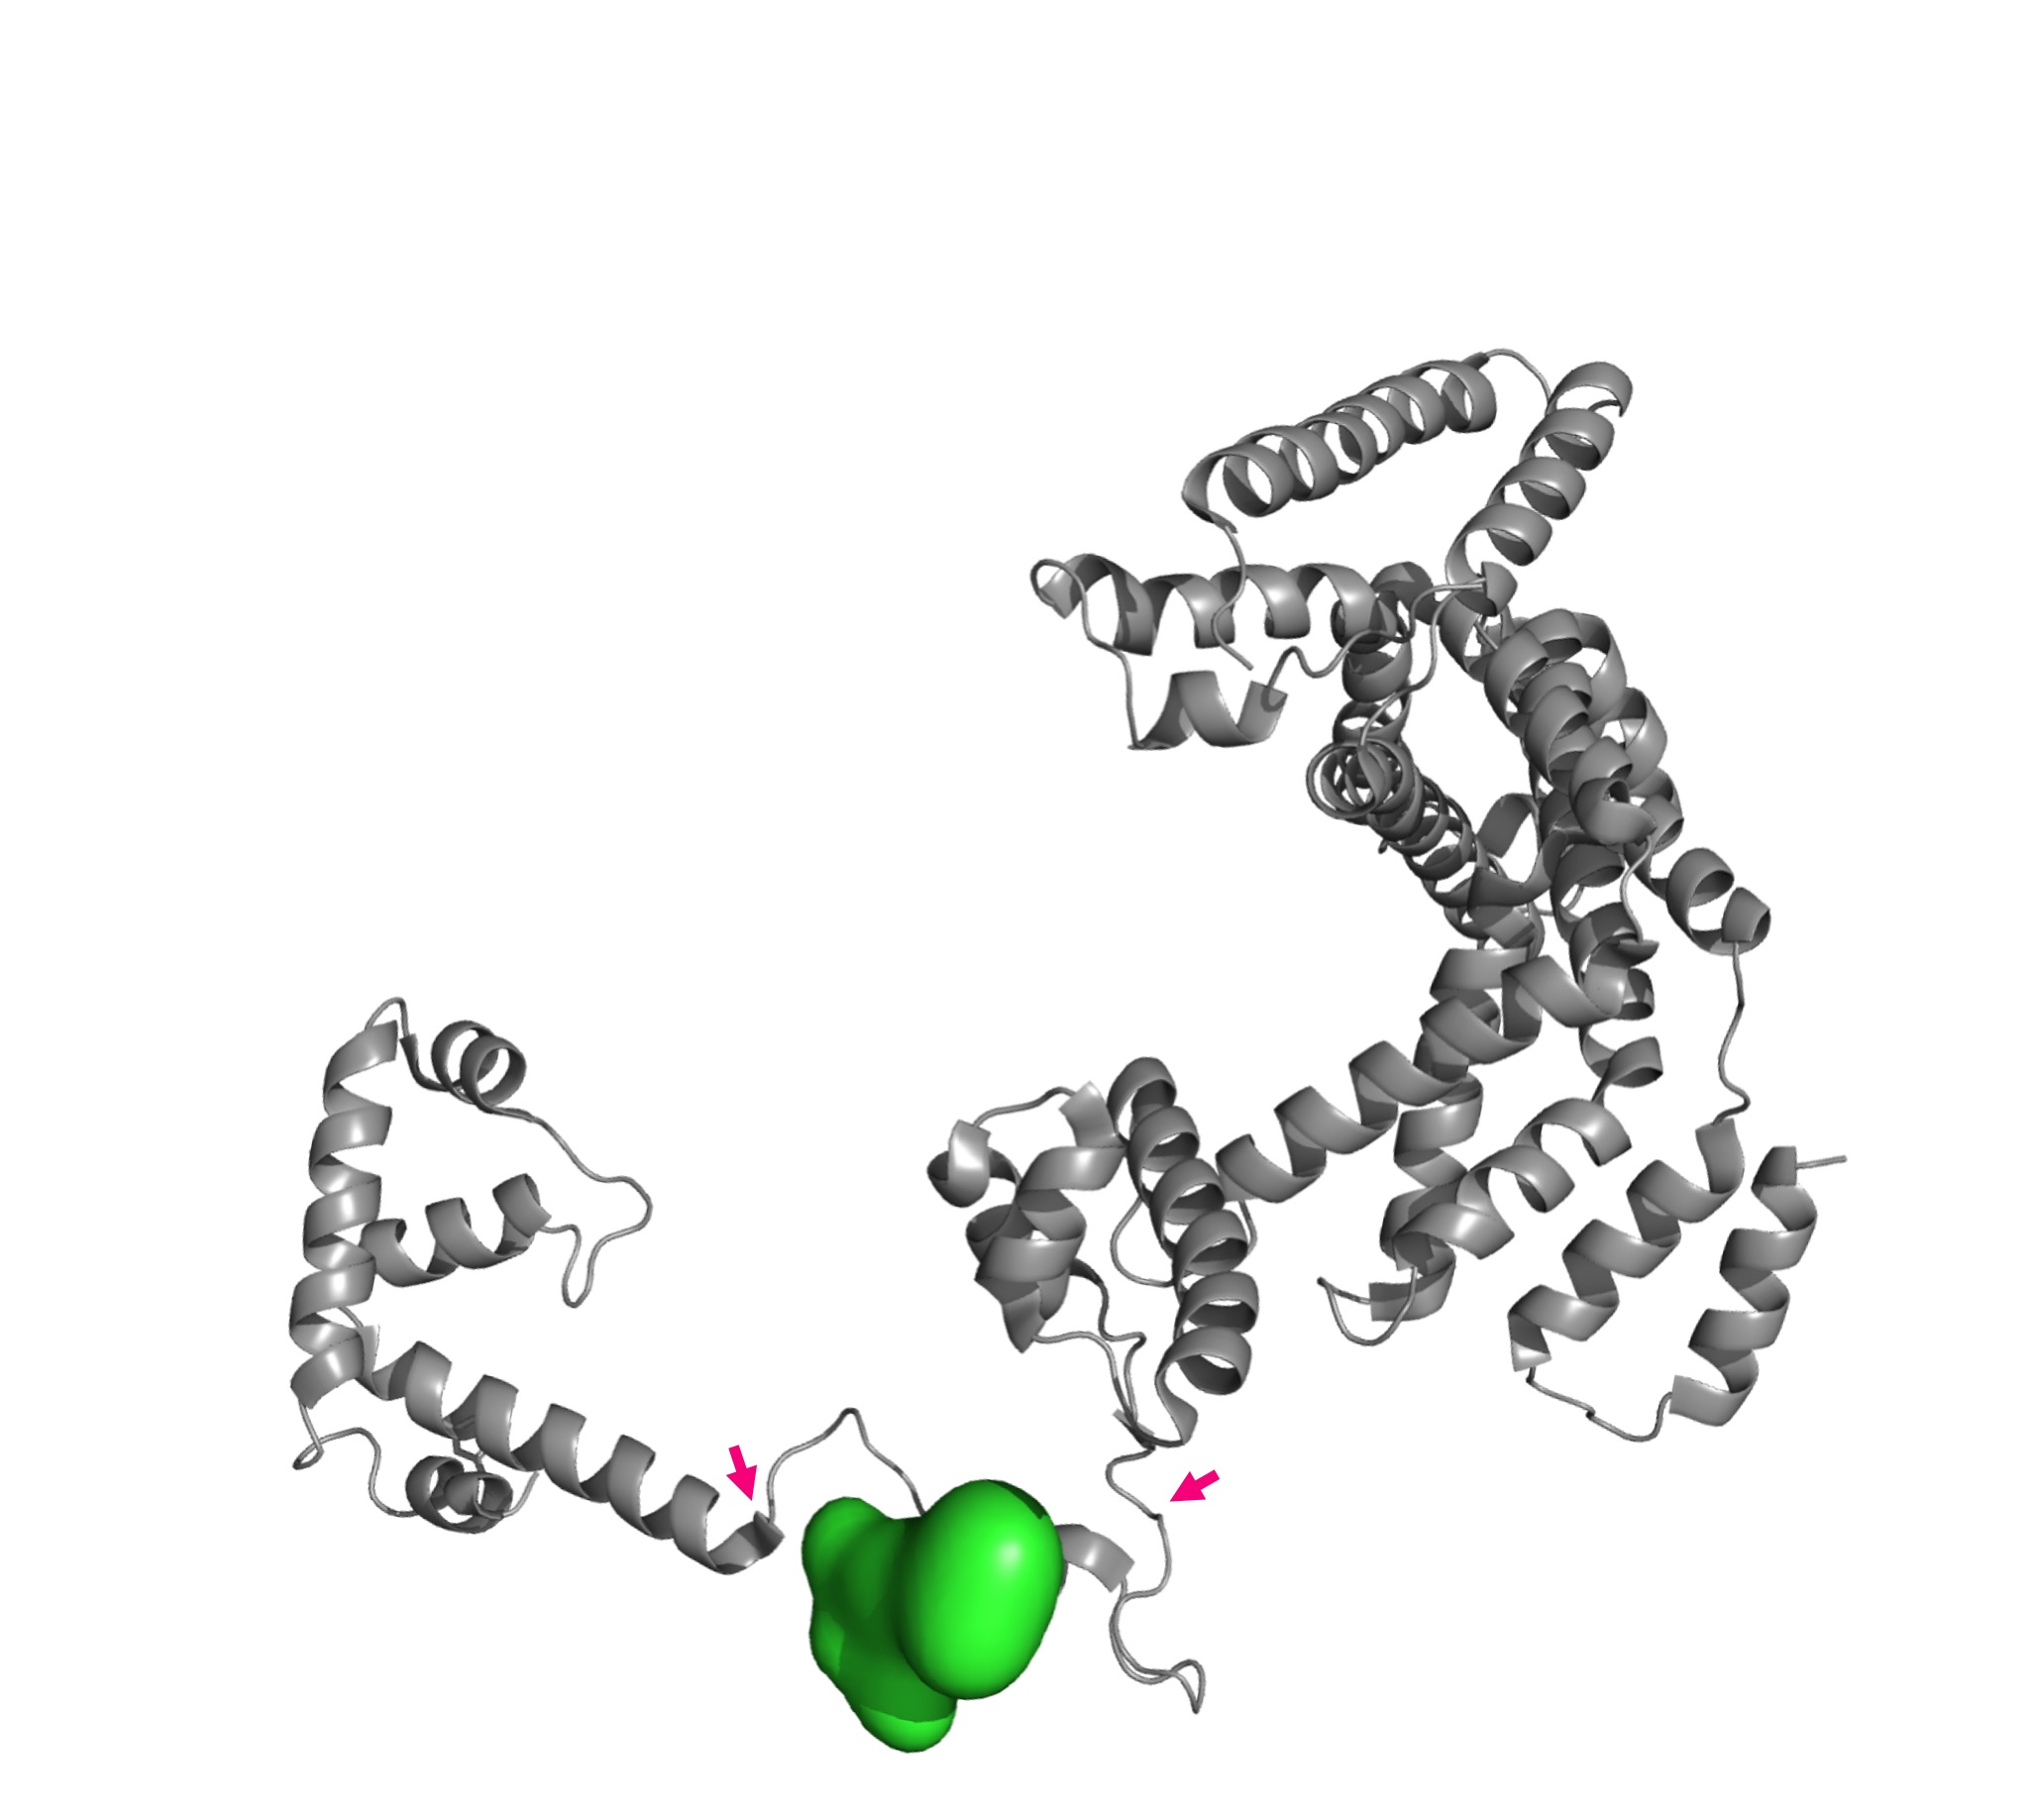
\includegraphics[width=\textwidth]{chapters/figures/sigma_3-2_loop_donor-dye.jpg}
    \caption{\label{fig:sigma_3-2_loop_donor-dye} 
    Donor-labeled $\sigma^{70}$ construct.
    The single-cysteine mutant (I511C) labeled with DyLight 550 via cysteine chemistry at the 511 amino acid position.
    The $\sigma^{70}$ factor is shown in grey and the $\sigma_{3.2}$ loop is indicated by magenta arrows.
    The accessible volume of the dye was modeled using the LabelLib software~\cite{dimura_NatComm_2020} in PyMol.
    PDB accession code 4YLN~\cite{zuo_steitz_2015}.
    }
\end{figure}

The TOP-10 cells that contained the pET28(+)-rpoD(+C) plasmid were selected by growing them on LB agar plates containing kanamycin. 
This step ensured that surviving TOP-10 colonies contained the rpoD(+C) insert, as indicated by the presence of the KanR gene. 
The selected colonies were then grown up in LB medium containing kanamycin to further ensure that only the plasmid containing cells would be used in the next step. 
The resulting pET28(+)-rpoD(+C) plasmids were extracted from the TOP-10 cells and purified through miniprep and subsequently sent for sequencing.
Sequencing results were used to verify that the point mutation was carried out successfully. 
The resulting plasmid library was then shared with collaborator Dr. Sergie Borukhov at Rowan University in New Jersey for protein overexpression, purification, and dye conjugation.
The current library consists of the following $\sigma^{70}$ single-cysteine mutants labeled with with DyLight550-maleimide: E508C, T509C, I511C, S517C, H518C, L519C, G520C, D546C, and K557C.

Figure~\ref{fig:sigma_3-2_loop_donor-dye} shows the $\sigma^{70}$-I511C construct labeled with a donor dye (DyLight 550) at the 511 amino acid position. 
The accessible volume of the donor dye was modeled using the LabelLib software, developed for course-grained simulation of fluorescent dyes in \ac{smFRET} experiments by the Seidel lab~\cite{dimura_NatComm_2020}.


\subsection{Design of acceptor-labeled \ac{lacCONS} constructs}
\label{sec:dsDNA_lib_exp}

In addition to labeling the $\sigma^{70}$ factor, we extended our labeling efforts to include the \ac{lacCONS} \ac{dsDNA} promoter sequence. 
In this case, we selectively attached the acceptor dye, ATTO647N, to specific positions on either the template strand or non-template strand of the \ac{dsDNA}.
An example of such a singly-labeled \ac{lacCONS} construct is depicted in Figure~\ref{fig:ds-lacCONS_seq}, where the label is positioned at $-28$ with respect to the \ac{ITS} on the non-template strand, denoted as $-28$NT.

The \ac{lacCONS} construct differs from the wt-\ac{lacCONS} in two important ways.
First, the \ac{ITS} where transcription of the nascent RNA begins (denoted by the $+1$ and an arrow in Fig.~\ref{fig:ds-lacCONS_seq}) is designed such that a partial set of \ac{NTP}s can be added to the transcription reaction stalling the reaction at specific time-points.
For instance, the addition of an ApA dinucleotide halts the reaction at $RP_{ITC=2}$ (Fig.~\ref{fig:ds-lacCONS_seq}).
In these experiments $RP_{ITC=2}$ represents a stable proxy for the open-bubble complex (\ac{$RP_o$}). 
If ApA and UTP are added, the system can be halted at $RP_{ITC=4}$. 
Furthermore, by introducing ApA, UTP, GTP, and ATP, we can induce stalling at $RP_e$, which corresponds to promoter escape. 
When a full set of \ac{NTP}s (UTP, GTP, ATP, and CTP) was added, the transcription reaction proceeded to completion, resulting in the generation of a full-length transcript.
However, the unlabeled nascent RNA is not detectable in \ac{smFRET} experiments. 

\begin{figure}
    \centering
    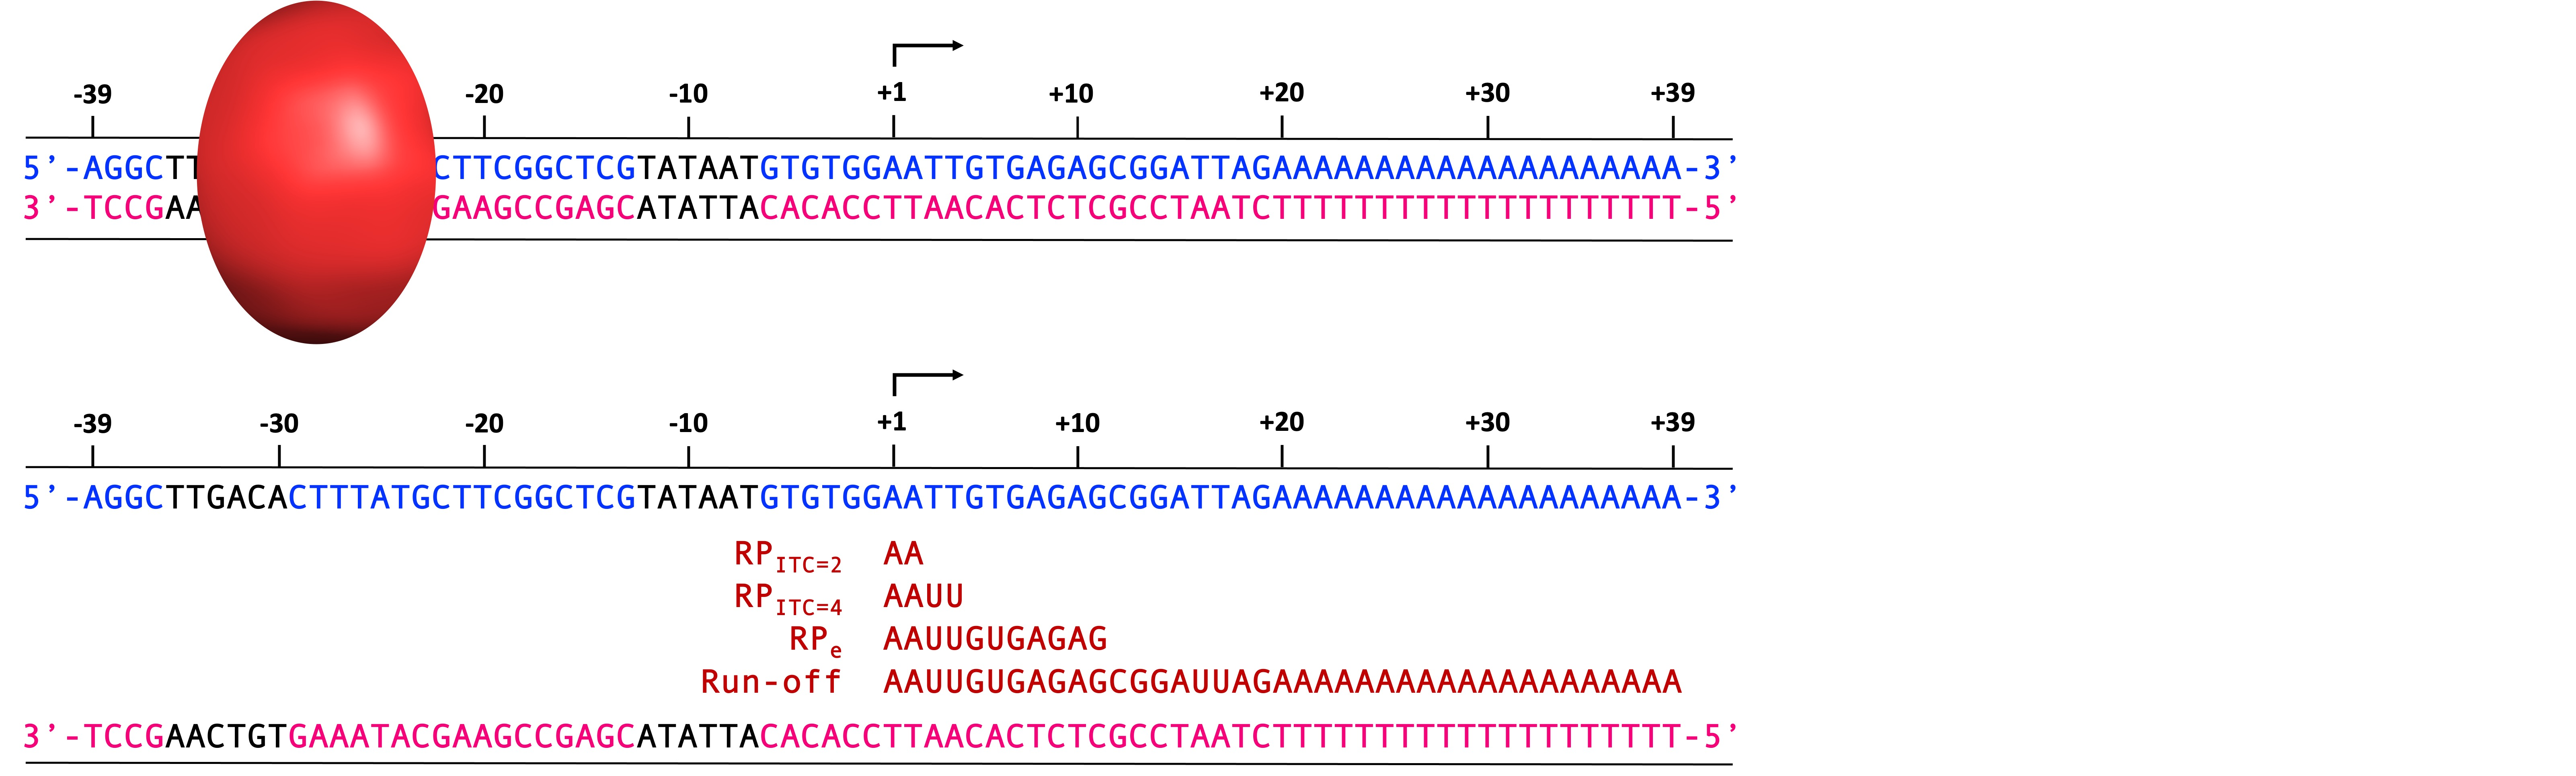
\includegraphics[width=1.5\textwidth]{chapters/figures/ds-lacCONS-seq.jpg}
    \caption{\label{fig:ds-lacCONS_seq} 
    \ac{dsDNA} template sequence based on the \ac{lacCONS} promoter.
    The non-template strand is presented in the 5' - 3' direction (blue), and the complementary template strand is presented the 3' - 5' direction (magenta).
    Top: lacCONS construct with an example acceptor dye (ATTO647N) labeled on the non-template strand at the -28 register, \textit{i.e.}, ($-28$NT). 
    The accessible volume of the dye is approximately to scale.
    Bottom: the \ac{ITS} of the wt-\ac{lacCONS} promoter was designed such that a partial set of \ac{NTP}s could be added and the transcription reaction could be stalled at specific points in the reaction, \textit{i.e.}, $RP_{ITC=2}$, $RP_{ITC=4}$, and $RP_{e}$ (nascent RNA transcripts indicated in red).
    A full-set of \ac{NTP}s results in run-off (transcription of the complete sequence).
    The full RNA transcript contains a 20dA sequence for binding to a 20dT \ac{ssDNA} labeled at each end with a donor and acceptor dye.
    The -35 element (-35 $-$ -30) and the TATA box (-12 $-$ -7 ) are indicated black.
    }
\end{figure}

\begin{figure}
    \centering
    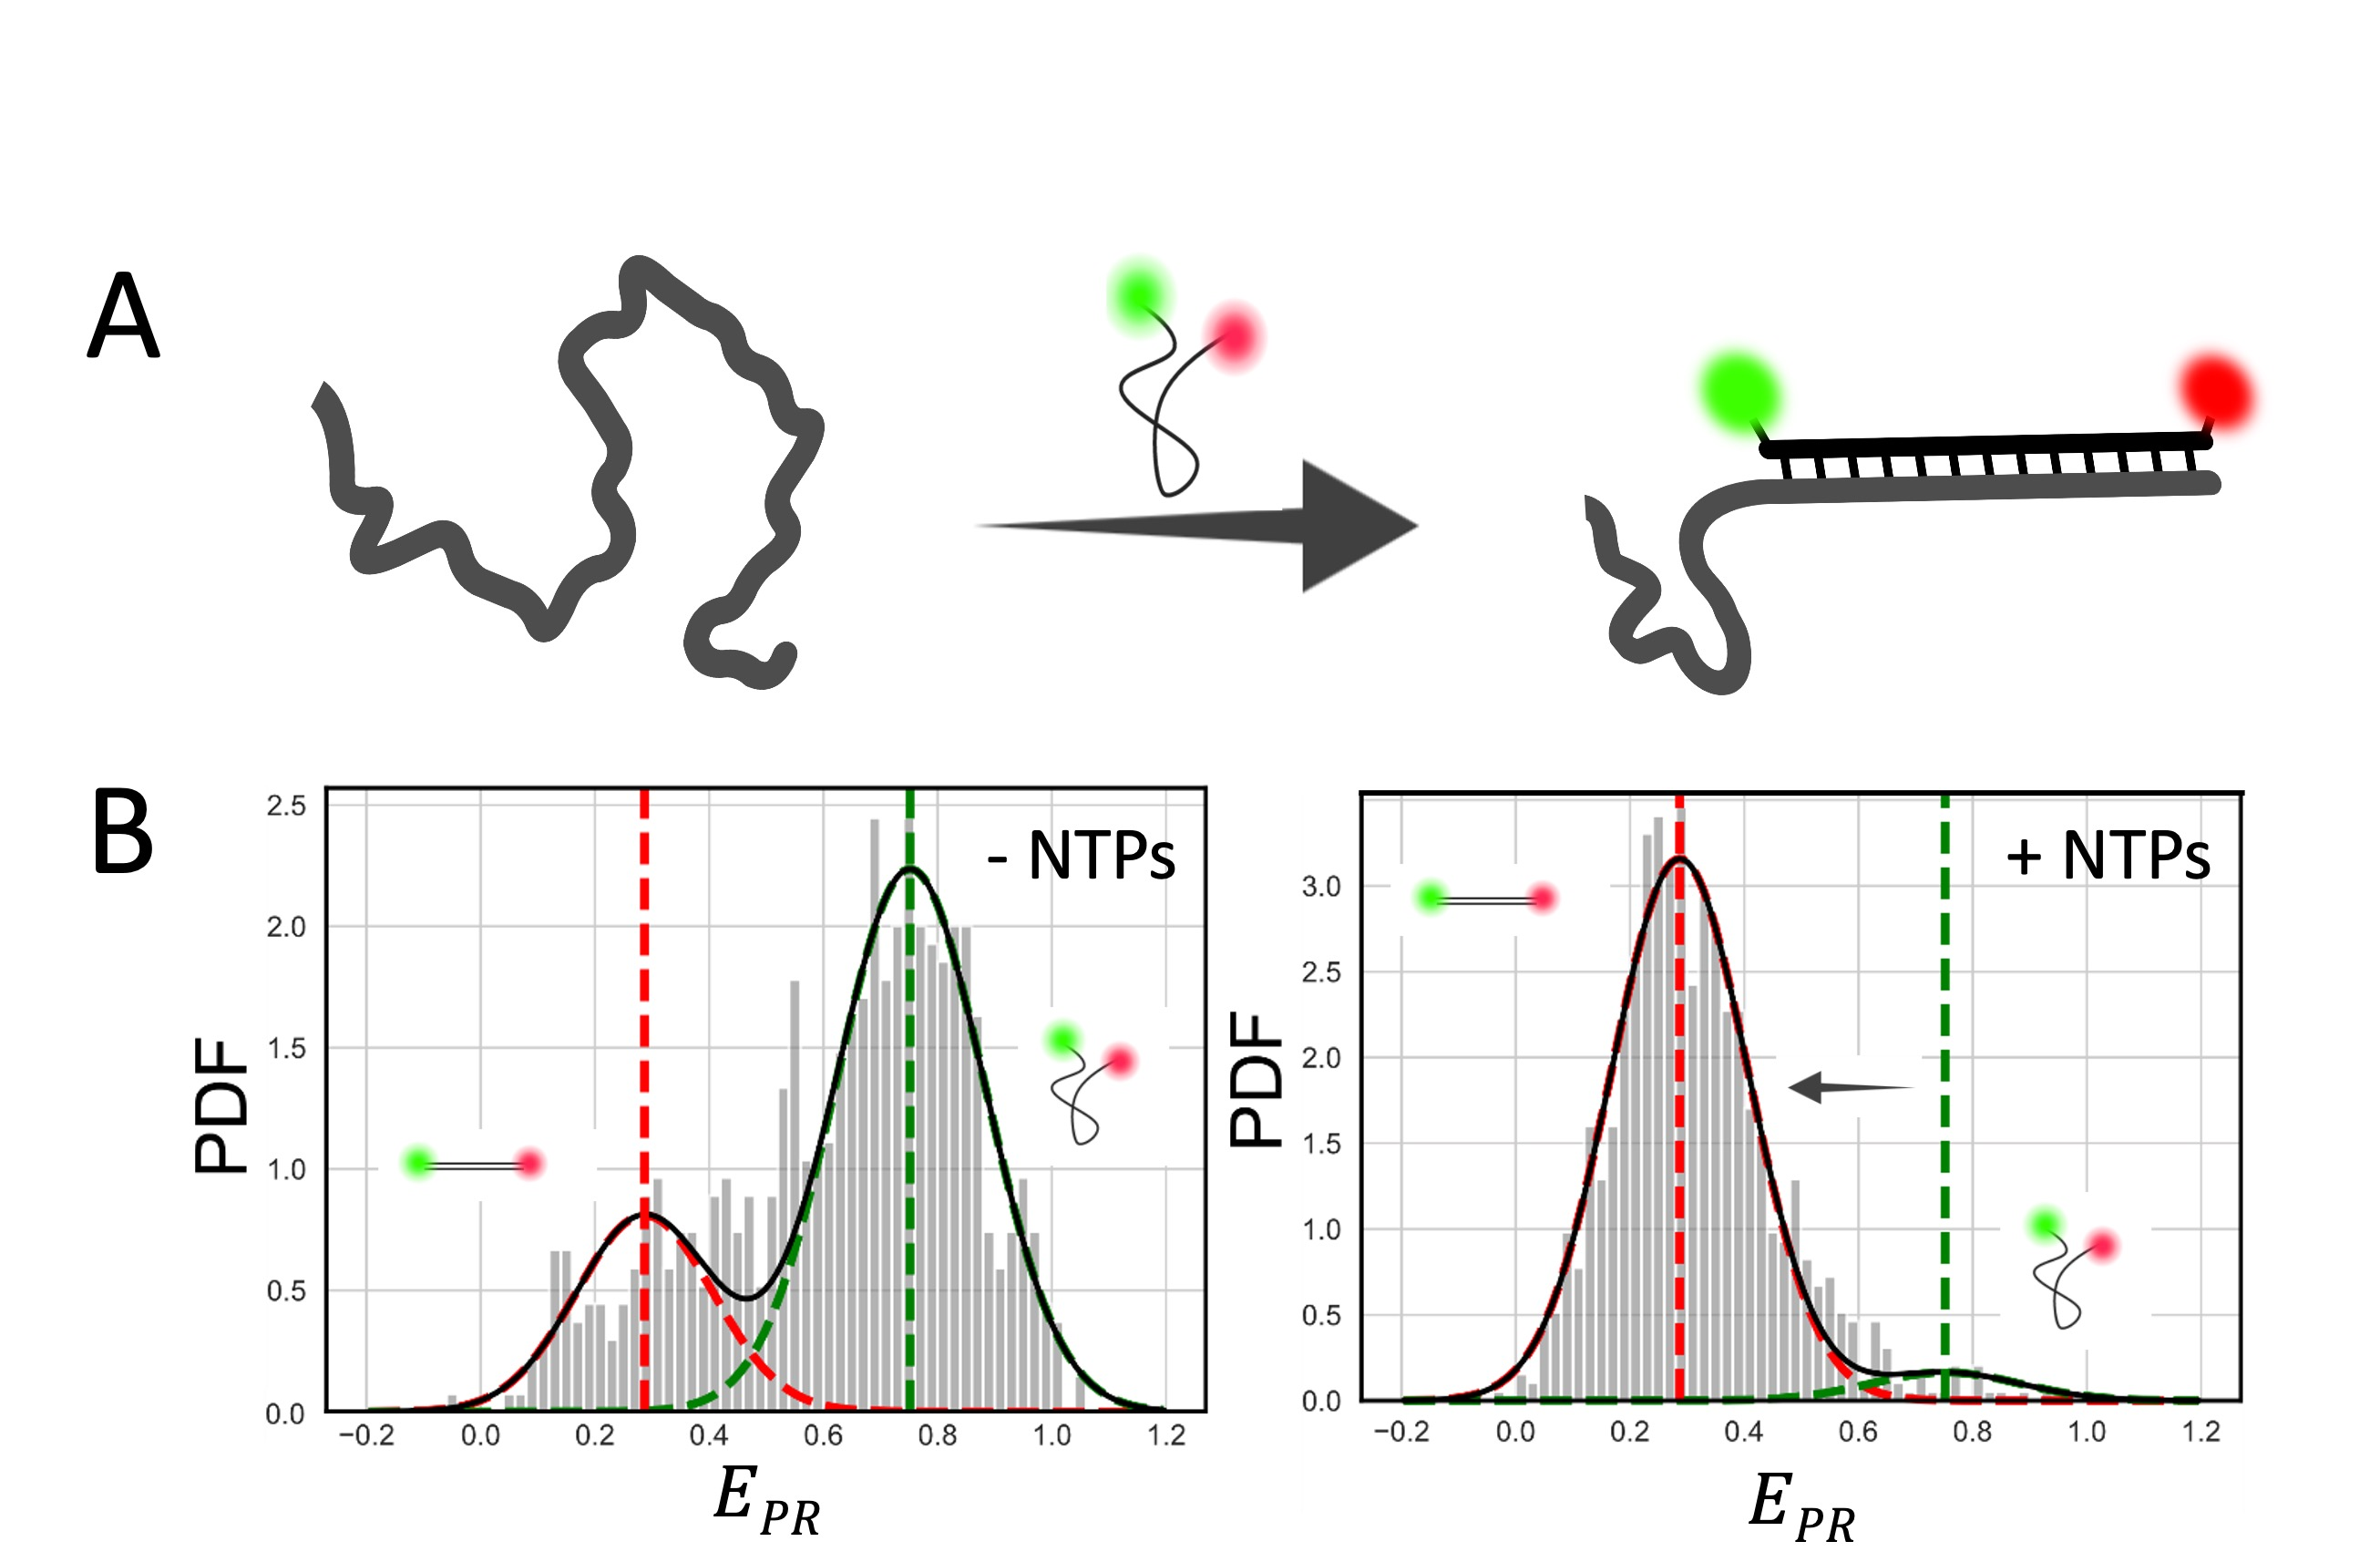
\includegraphics[width=\textwidth]{chapters/figures/probe_binding_assay.jpg}
    \caption{\label{fig:probe-binding_assay} 
    Probe-binding assay.
    A) After transcription is complete, the final product is a nascent RNA (grey worm-like chain). Note that the nascent RNA is unlabeled and therefor is not detectable in \ac{smFRET} experiments. 
    When a \ac{ssDNA} 20dT FRET-probe is added to solution, it readily binds the 20~\ac{bp} poly-A tail of the nascent RNA. 
    B) FRET histograms for the probe-binding assay
    The histogram on the left shows two distinct FRET populations in the absence of \ac{NTP}s, where the low-FRET populations corresponds to the bound 20dT FRET-probe, and the high-FRET populations corresponds to the unbound 20dT FRET-probe. 
    This result suggests that the transcription reaction did not go to completion. 
    The histogram on the right shows the shift if FRET populations upon addition of a full set of \ac{NTP}s. 
    The shift of the distributions (left-pointing black arrow) clearly indicates that nearly all of the FRET-probe is bound to nascent RNA from the completed transcription reaction.
    }
\end{figure}

To verify the presence of full-length RNA transcripts and to ensure that the transcription reaction reached completion, we introduced a \enquote{probe-binding} sequence into the \ac{lacCONS} construct.
Figure~\ref{fig:ds-lacCONS_seq} shows a full-transcript (run-off) featuring a poly-A tail, referred to throughout as a \enquote{20dA} sequence.
In end-point \ac{smFRET} experiments, after the transcription reaction has gone to completion and 600~mM guanidinium chloride (GdmCl) has been added to quench the reaction, a specialized \enquote{FRET-probe} is introduced.
This 20dT \ac{ssDNA} is labeled at both ends with a donor and an acceptor dye and binds the 20dA sequence of the nascent RNA, as illustrated in Figure~\ref{fig:probe-binding_assay}A.
By adding this doubly-labeled FRET-probe, we were able to detect the presence of the nascent RNA, as the bound probe and the unbound probe correspond to two distinct FRET populations, as shown in Figure~\ref{fig:probe-binding_assay}B. 
The high FRET populations correspond to the unbound, highly flexible 20dT probe, and the low FRET population corresponds to the 20dT probe bound to the nascent RNA.
By performing this experiment both in the presence and absence of \ac{NTP}s we can quantify the amount of RNA produced in a given transcription reaction. 

\section{FRET distance measurement network}
\label{sec:distance_network_exp}

Conventional structural determination methods offer only snapshots of molecules in motion, making them inadequate for capturing the dynamic behavior of complex enzymes like \ac{RNAP}.
In addition, common methods such as crystallization or cryo-EM require non-native conditions, which may introduce artifacts when solving structures. 
To overcome this limitation, we will utilize freely-diffusing \ac{RNAP} in conjunction with a new 32-spot \ac{HT-smFRET} setup, coupled with a rapid microfluidic mixer. 
This new platform will enable us to observe the entire process of promoter escape in real-time, providing valuable insights into the enzyme's dynamic mechanisms.

FRET data is inherently sparse due to labeling position constraints~\cite{kalinin_NatMethods_2012, muschielok_NatMethods_2008}, as introduction of a bulky fluorescent dye may either not be possible or may interfere with a molecule's native function. 
% In addition, making the comprehensive single-cysteine library is time consuming.
% Together, these factors make it difficult to capture the full spectrum of structural details using \ac{smFRET} alone. 
In order to overcome this limitation, structural determination using FRET distance measurement networks~\cite{hellenkamp_NatMethods_2017} can be augmented by integrating computer simulations.
This combination of experimental and computational approaches provides a more comprehensive method for exploring biomolecular structures and enables access to microsecond timescale dynamics~\cite{lerner_Science_2018, dimura_COSB_2016, kilic_NatComm_2018, dimura_NatComm_2020}.

In my thesis work, I have established the foundation for constructing a \ac{smFRET} distance network between the acceptor-labeled \ac{lacCONS} promoter library and the donor-labeled $\sigma^{70}$ library. 
This involves systematic observations of the $\sigma^{70}$ mutants in relation to the library of singly-labeled \ac{dsDNA} \ac{lacCONS} promoters. 
The data derived from these experiments will serve as constraints in molecular simulations~\cite{dimura_COSB_2016}, enabling detailed studies of the structural dynamics governing the interactions between \ac{RNAP} and DNA throughout the promoter escape process.
For clarity, Figure~\ref{fig:distance_network}A illustrates a partial distance network for the $\sigma^{70}$-I511C construct and the template strand only. 
The full distance network will involve many more distances derived from the $\sigma^{70}$ and \ac{dsDNA} libraries.
Table~\ref{tab:labeling_positions} shows all the possible labeling positions on the template and non-template strands of the \ac{lacCONS} promoter as well as the library of labeled $\sigma_{3.2}$ constructs.
The total possible number of distances is then $78 \times 78 \times 9 = 54,759$.
An example of a single distance measurement is presented in Figure~\ref{fig:distance_network}B, where an acceptor dye is labeled at the $-28$NT position and a donor dye is labeled on the $\sigma_{3.2}$-I511C construct. 
Note that the accessible volume of the donor dye is not continuous, as the LabelLib software constrains the volume based on the existing structure of the flexible $\sigma_{3.2}$ loop. 

\begin{figure}
    \centering
    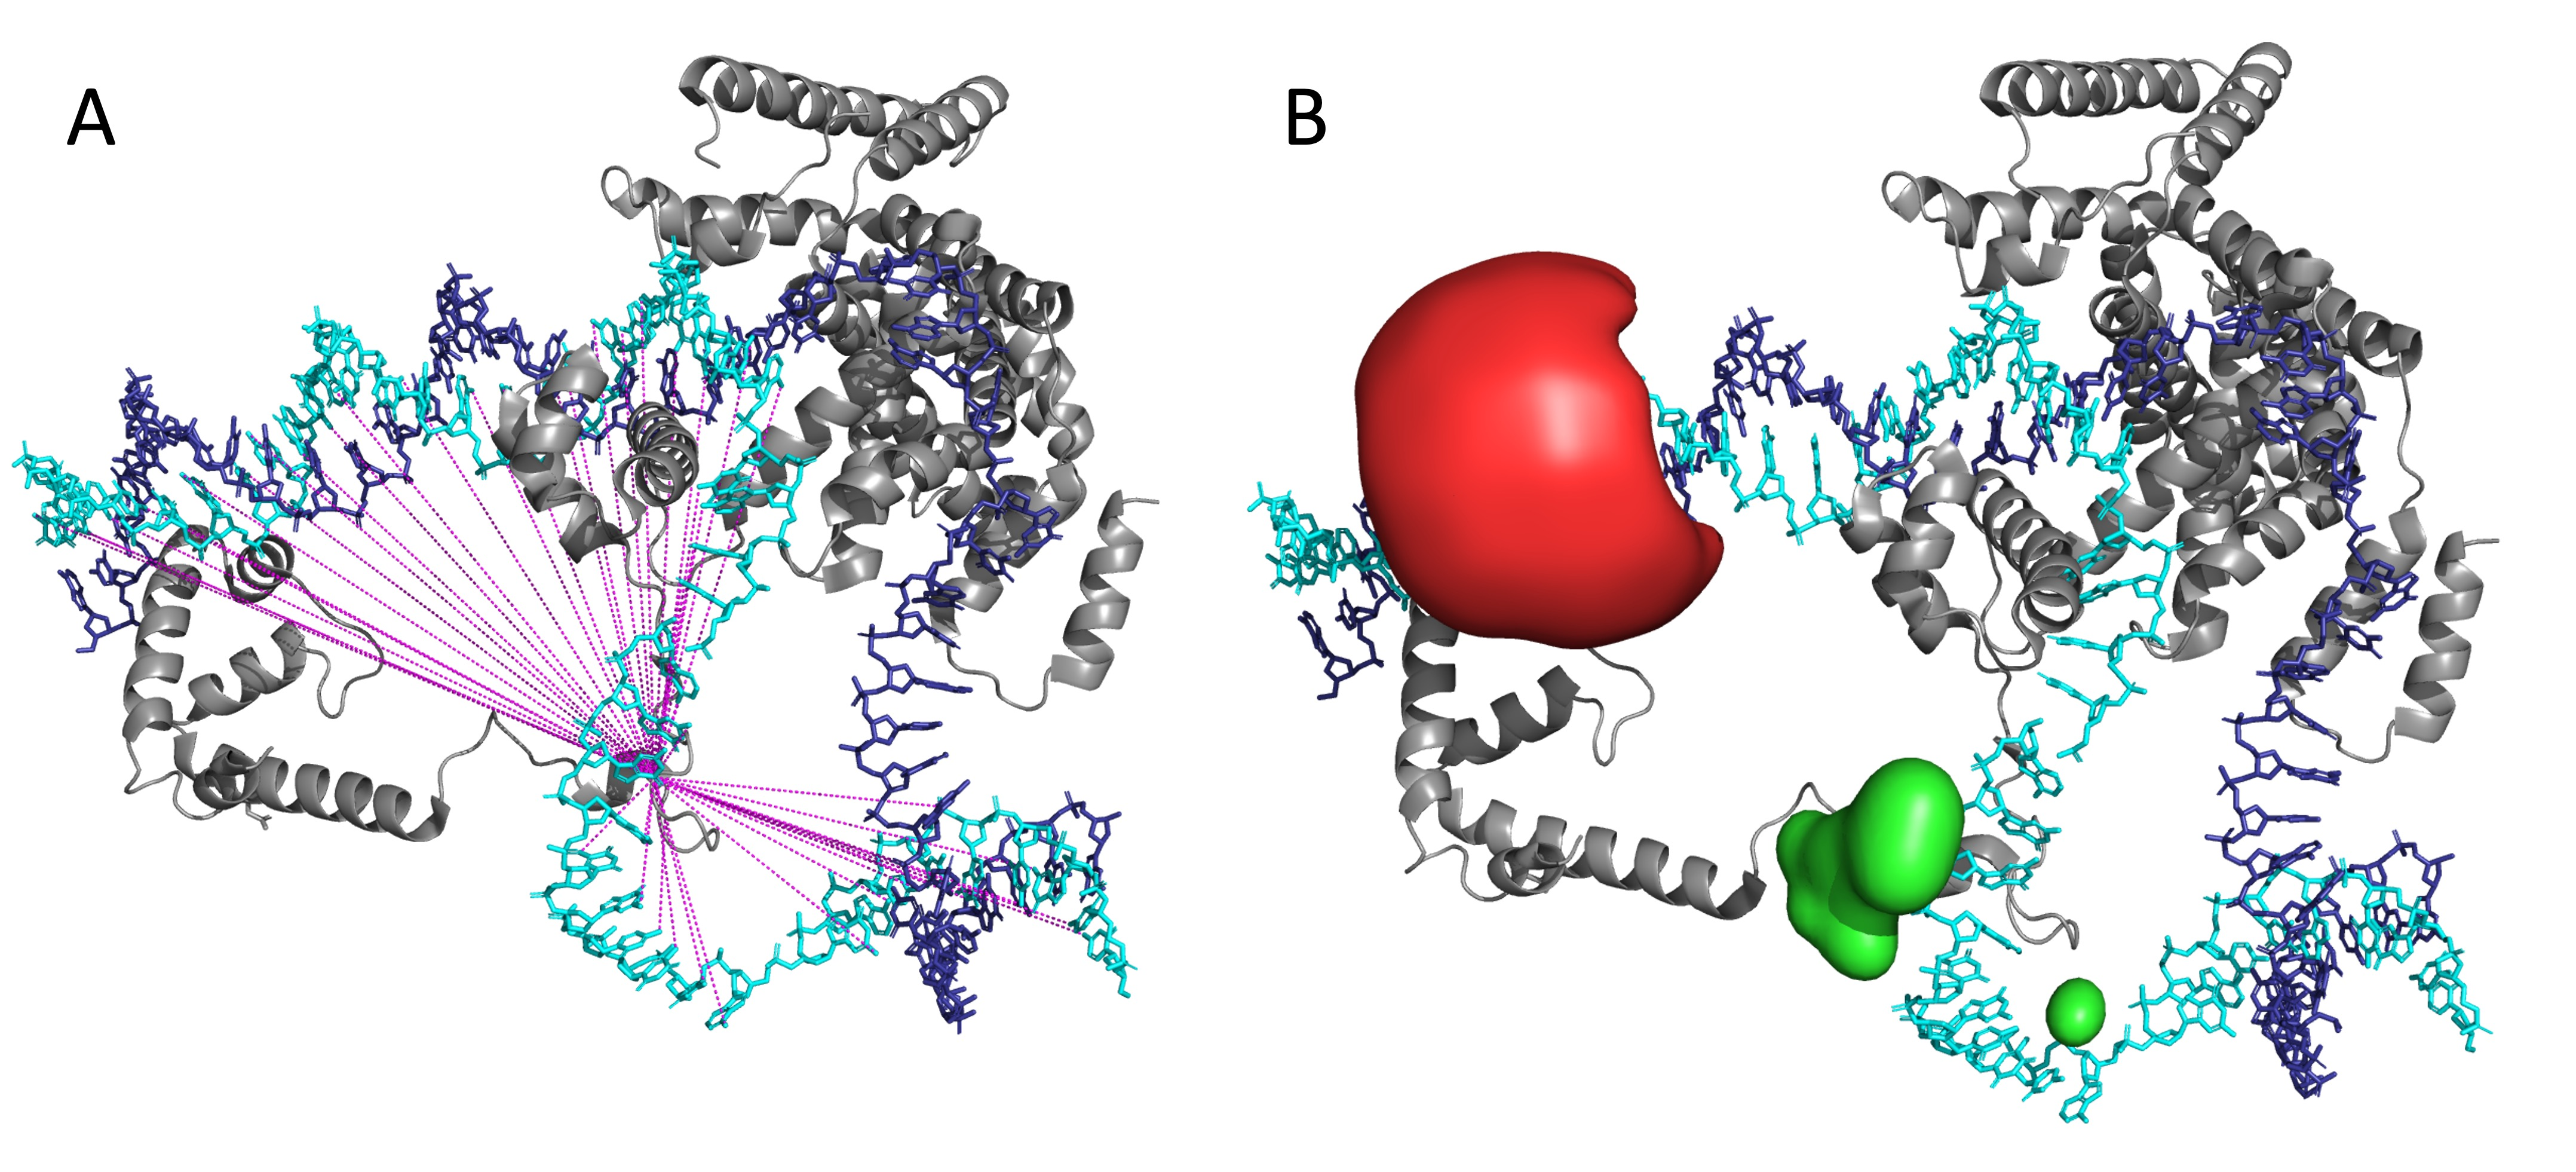
\includegraphics[width=\textwidth]{chapters/figures/distance_network.jpg}
    \caption{\label{fig:distance_network} 
    FRET distance measurement network and accessible volumes of FRET-labeled $\sigma^{70}$-\ac{dsDNA} complex.
    A) The $\sigma^{70}$ factor (grey) bound to the \ac{lacCONS} promoter in an open-bubble conformation.
    The non-template strand is shown in cyan and the template strand is shown in navy blue. 
    Distances are indicated by magenta dashed lines between locations in the non-template strand and the 511 amino acid position of $\sigma^{70}$-I511C.  
    Note that this measurement network shows only distances from a single mutant to distances on the non-template strand of the \ac{lacCONS} promoter.
    A complete distance network includes all of the transcriptionally active mutants in the library against all of the compatible locations on the \ac{dsDNA}.
    B) Accessible volume of the donor-labeled (green) $\sigma_{3.2}$ loop at the 511 position.
    Accessible volume of the acceptor-labeled (red) \ac{lacCONS} promoter at the -28 position on the non-template strand. 
    Accessible volumes generated using the LabelLib software~\cite{dimura_NatComm_2020}
    PDB accession code 4YLN~\cite{zuo_steitz_2015}.
    }
\end{figure}

\begin{table}[]
\centering
\caption{Labeling positions for the donor-labeled $\sigma^{70}$ library and the acceptor-labeled \ac{lacCONS} library.}
\label{tab:labeling_positions}
\begin{tabular}{@{}lllllllll@{}}
\toprule
\multicolumn{4}{c}{\textbf{Template}} & \multicolumn{4}{c}{\textbf{Non-template}} & \textbf{$\sigma_{3.2}$} \\ \midrule
-39     & -19     & +01     & +21     & -39      & -19      & +01      & +21      & 508                     \\
-38     & -18     & +02     & +22     & -38      & -18      & +02      & +22      & 509                     \\
-37     & -17     & +03     & +23     & -37      & -17      & +03      & +23      & 511                     \\
-36     & -16     & +04     & +24     & -36      & -16      & +04      & +24      & 517                     \\
-35     & -15     & +05     & +25     & -35      & -15      & +05      & +25      & 518                     \\
-34     & -14     & +06     & +26     & -34      & -14      & +06      & +26      & 519                     \\
-33     & -13     & +07     & +27     & -33      & -13      & +07      & +27      & 520                     \\
-32     & -12     & +08     & +28     & -32      & -12      & +08      & +28      & 546                     \\
-31     & -11     & +09     & +29     & -31      & -11      & +09      & +29      & 557                     \\
-30     & -10     & +10     & +30     & -30      & -10      & +10      & +30      &                         \\
-29     & -9      & +11     & +31     & -29      & -9       & +11      & +31      &                         \\
-28     & -8      & +12     & +32     & -28      & -8       & +12      & +32      &                         \\
-27     & -7      & +13     & +33     & -27      & -7       & +13      & +33      &                         \\
-26     & -6      & +14     & +34     & -26      & -6       & +14      & +34      &                         \\
-25     & -5      & +15     & +35     & -25      & -5       & +15      & +35      &                         \\
-24     & -4      & +16     & +36     & -24      & -4       & +16      & +36      &                         \\
-23     & -3      & +17     & +37     & -23      & -3       & +17      & +37      &                         \\
-22     & -2      & +18     & +38     & -22      & -2       & +18      & +38      &                         \\
-21     & -1      & +19     & +39     & -21      & -1       & +19      & +39      &                         \\
-20     &         & +20     &         & -20      &          & +20      &          &                         \\
\bottomrule
\end{tabular}
\end{table}

However, not all $\sigma^{70}$ mutants will be transcriptionally active, and not all doubly-labeled protein-DNA complexes will be compatible and informative. 
As a result, we will conduct distance measurements for informative pairs of transcriptionally active mutants and compatible acceptor-labeled \ac{lacCONS} promoters.
To optimize the experimental design for informative pairs and minimize the number of required experiments, I have employed modeling techniques using the LabelLib software~\cite{dimura_NatComm_2020} to define accessible volumes of the dyes at specific locations on the $\sigma_{3.2}$ loop.
Using the accessible volumes it is also possible to estimate a mean FRET efficiency and the corresponding inter-dye distance. 
This step helps to identify and prioritize scenarios that are more likely to yield valuable insights, as outlined in Demura \textit{et al.,} 2020.~\cite{dimura_NatComm_2020}

In addition, the subsequent screening process, explained in the next section, will significantly narrow down the pool of experiments required.
Only those complexes that successfully pass modeling and screening will contribute to the final FRET distance network, which will then serve as the basis for generating FRET-restrained simulations.

\section{Control measurements on the single-spot ALEX setup}
\label{se:controls_exp}

Control experiments are an integral part of this approach, serving to validate and refine the \ac{HT-smFRET} methodology. 
Notably, we perform these experiments on the single-spot $\mu$s\ac{ALEX} setup in order to ensure comparability between setups.
Two important control experiments must be carried out.
First, the $\sigma^{70}$ constructs must be tested for transcriptional activity, and second, the acceptor-labeled \ac{lacCONS} promoters must be tested for compatibility with the active $\sigma^{70}$ constructs. 

In the initial series of control experiments, I assessed the transcriptional activity of the $\sigma^{70}$ mutants using the previously described probe-binding assays. 
A summary of the results of this screening for the nine constructs in the $\sigma^{70}$ library are presented in Figure~\ref{fig:mutant_screening} (constructs that did not pass the screening are not shown).
In these experiments, we distinguished two populations based on their FRET signals. 
The bound population, representing the low-FRET state, corresponds to the nascent RNA bound to the probe. 
The unbound population, characterized by the high-FRET state, corresponds to the free probe. 
Upon the addition of \ac{NTP}s, the distributions shifted from primarily high-FRET to predominantly low-FRET populations. 
Only mutants demonstrating activity in this assay proceeded to the next phase of screening.

At this stage, only two of the $\sigma^{70}$ constructs, namely $\sigma^{70}$-I511C and $\sigma^{70}$-519C, exhibited transcriptional activity and successfully passed the initial screening. 
This observation underscores the sensitivity of the $\sigma_{3.2}$ loop and its critical role in promoter escape. 
As we continue our investigations, we may explore additional positions in and around the $\sigma_{3.2}$ loop.

In the second set of control experiments, we perform open-bubble experiments using a singly-labeled $\sigma^{70}$ that passed the first test with a singly-labeled \ac{lacCONS} promoter. 
In these experiments we measure the changes in distance between \ac{RNAP} and the \ac{dsDNA} using a partial set of \ac{NTP}s as described in Section~\ref{sec:dsDNA_lib_exp}.
If we observe normal behavior, these FRET pairs will be used in \ac{HT-smFRET} experiments on the new 32-spot platform for kinetic studies of the promoter escape reaction. 

\begin{figure}
    \centering
    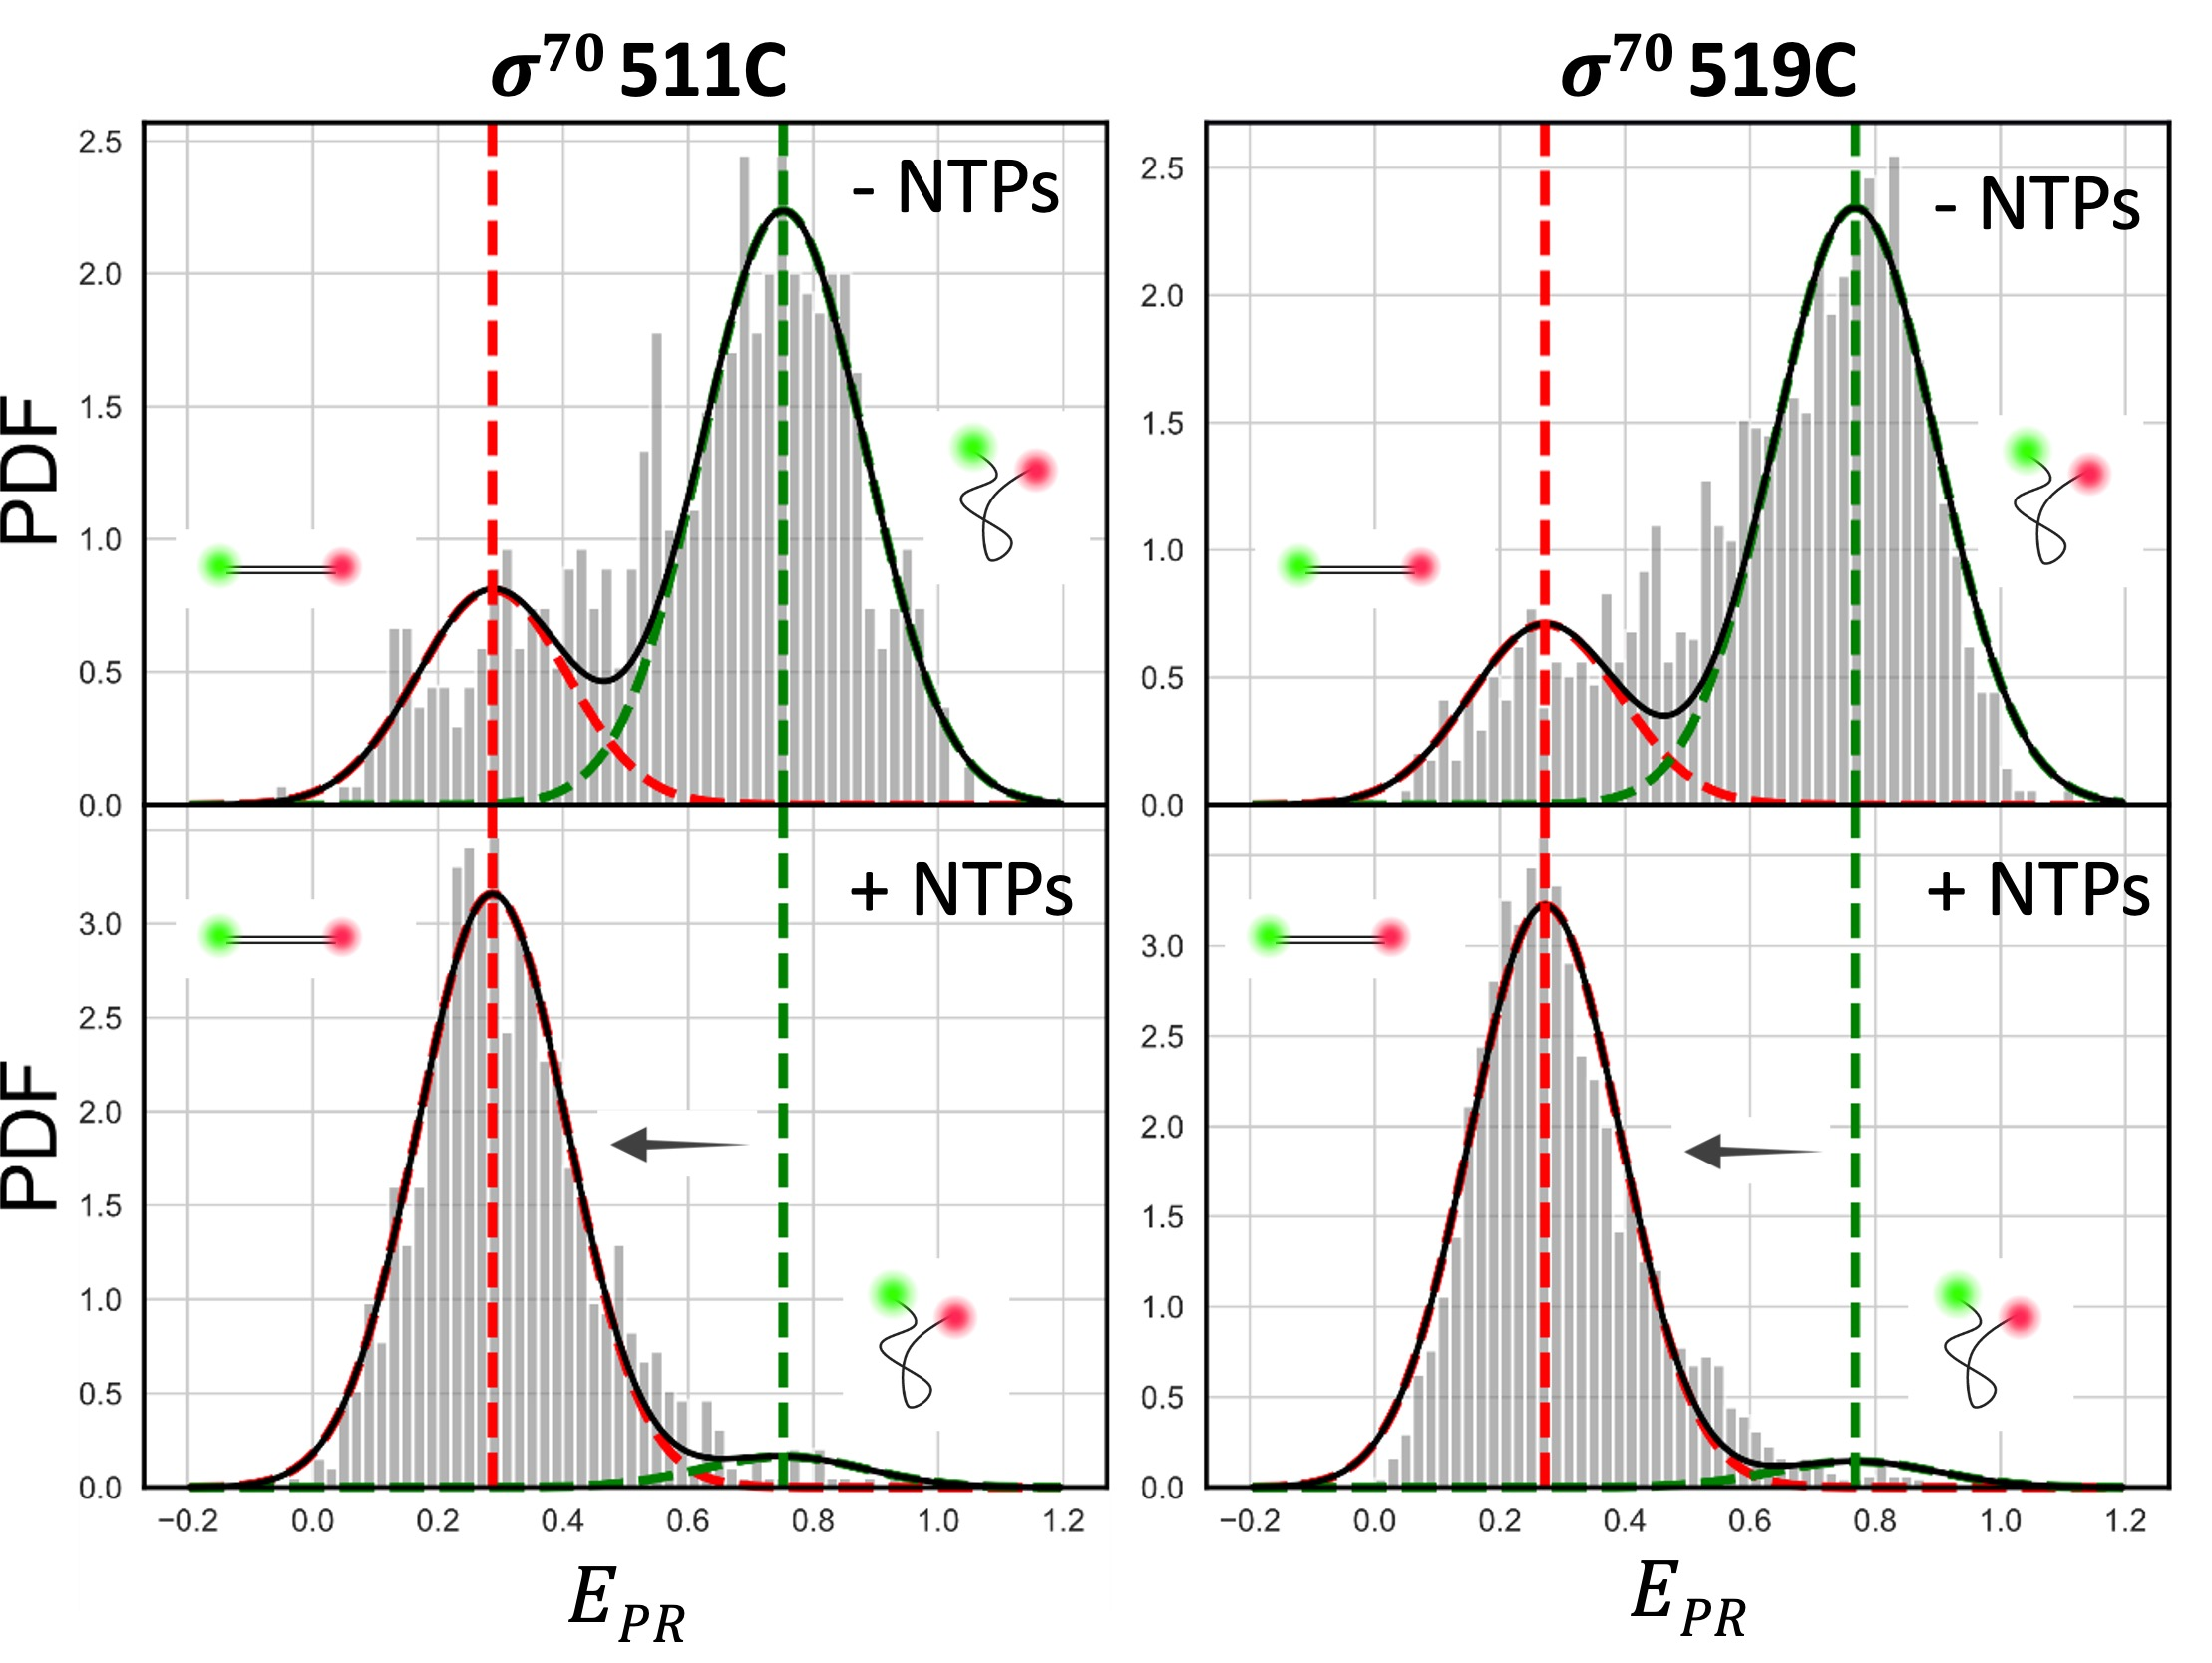
\includegraphics[width=\textwidth]{chapters/figures/mutant_screening_hists.jpg}
    \caption{\label{fig:mutant_screening} 
    Proximity ratio histograms of the probe-binding assay. 
    The $\sigma^{70}$ mutant library was screened for transcriptional activity using a probe-binding assay using the 20dT probe. 
    $\sigma_{3.2}$ constructs labeled with DyLight 550 at the 511 and 519 positions were tested in the absence (-NTPs) and the presence (+NPTs) of a full set of NTPs.
    The reactions were quenched using 600~mM GdmCl and the 20dT FRET probe was added.
    }
\end{figure}


\section{Real-time kinetics of promoter escape using an improved HT-smFRET platform}
\label{sec:HT-smFRET_of_txn_exp}

Expanding on the concept of utilizing \ac{smFRET}-derived distances as constraints for molecular dynamics or coarse-grained simulations, we will incorporate distance constraints that evolve over time during a reaction.
These collections of both static structures and dynamic distance constraints will be incorporated into an energy cost function using a course-grained simulation framework. 
The outcome will be the creation of 3D atomic-level structural dynamic representations, effectively capturing the dynamic behavior of these molecules as they perform their biological functions.

\subsection{Next generation multi-spot platform with a fast microfluidic mixer}
\label{sec:32-spot_intro}

In the next step of this work, we will transition from the initial single-spot experiments to a cutting-edge 32-spot \ac{HT-smFRET} platform equipped with a fast microfluidic mixer. 
This transition marks a significant advancement in our research, enabling us to capture real-time kinetic data on the entire promoter escape reaction.

The 32-spot setup is equipped with two 1~W \ac{CW} lasers and employs $\mu$s\ac{ALEX}. 
It incorporates two linear $32\times1$ \ac{SPAD} arrays, which have been fabricated using red-enhanced technology. 
This technological advancement significantly improves sensitivity, particularly in the acceptor spectral band, as highlighted in Ceccarelli \textit{et al.,} 2018\cite{ceccarelli_IEEEPTL_2018}.

Similar to the 8-spot setup, the 32-spot microscope adopts a linear excitation pattern generated using a cylindrical lens. 
This modification offers advantages in terms of cost-effectiveness and ease of operation. In particular, alignment is considerably simplified compared to the previous pattern generation technique involving \ac{LCOS-SLM}.

To validate the 32-spot setup, we will initially utilize fluorescently labeled \ac{dsDNA}, followed by the labeled RNAP-Promoter complexes in equilibrium. 
These initial results will be compared to control measurements obtained using the single-spot \ac{ALEX} setup. 
Once validation is complete, we will proceed with the installation of the microfluidic mixer, which has been expertly designed by the Schuler group at the University of Zurich.

\begin{figure}
    \centering
    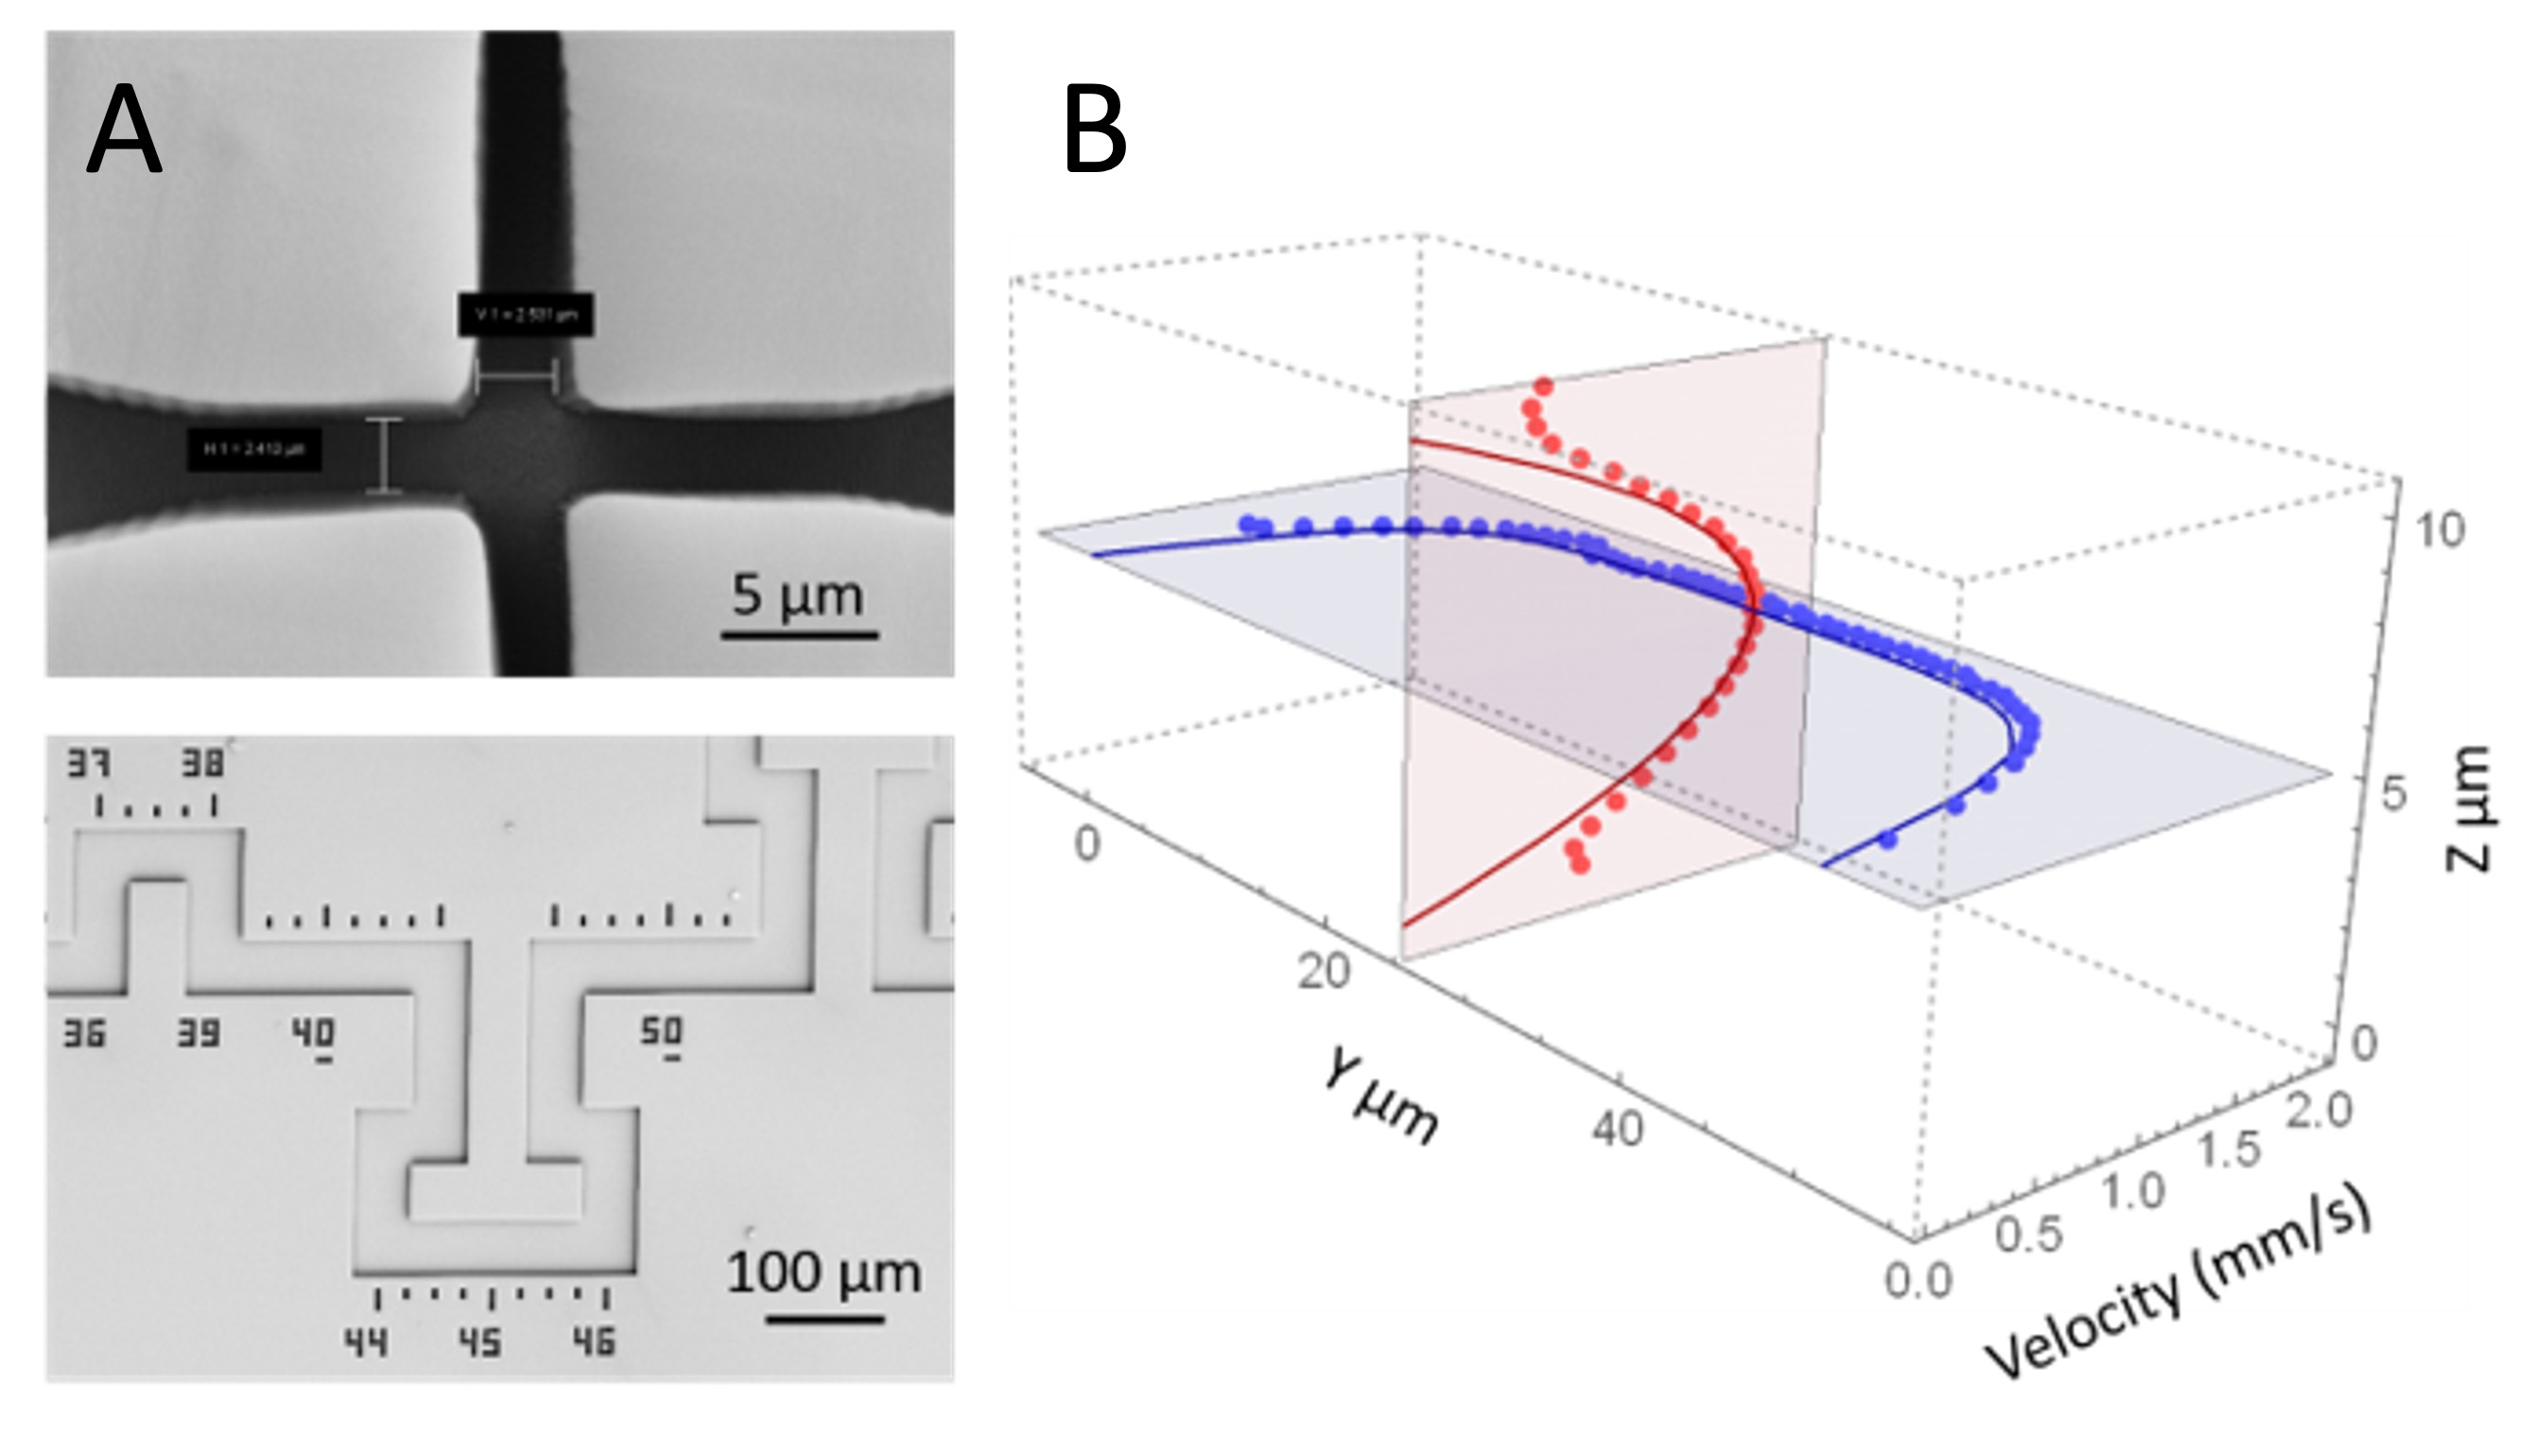
\includegraphics[width=\textwidth]{chapters/figures/schuler_mixer.jpg}
    \caption{\label{fig:schuler_mixer} 
    A) Scanning electron microscopy was used to obtain images of the mixing (top) and observation regions (bottom). 
    B) Flow velocities in the microfluidic device were determined using two-focal \ac{FCS} measurements of a flowing sample of AlexaFluor 488 indicated by red and blue dots.
    Finite-element calculations are indicated by solid red and blue lines in the Y-Z and X-Z planes respectively.
    }
\end{figure}

These microfluidic mixers have been carefully designed to facilitate the investigation of fast biomolecular kinetics under non-equilibrium conditions using the $32\times1$ \ac{SPAD} arrays. 
These mixers employ laminar hydrodynamic focusing and rapid diffusive mixing and have undergone optimization for the desired mixing ratios and flow velocities through extensive 3D finite-element calculations (COMSOL Multiphysics 5.2). 
With this design, a mixing dead time of approximately 1~ms is achievable. 

Figure~\ref{fig:schuler_mixer}A shows scanning electron micrographs of the mixing (top) and observation (bottom) regions within the mixer. 
A serpentine observation channel has been designed to accommodate a broad range of observation times and enable multifocal detection along the central channel using the linear 32-spot arrays, (bottom of Fig.~\ref{fig:schuler_mixer}A).

To ensure the production of reliable devices with stable flow patterns and highly reproducible mixing behavior, the Schuler group emploed microfabrication techniques based on reactive ion etching in silicon to create precise device molds. 
This precision is critical for achieving fast diffusive mixing in the narrow channels (2.5~$\mu$m). 
The microfluidic devices are fabricated by filling the molds with \ac{PDMS} and bonding them to microscope cover glasses following plasma activation. 
To control the flow rate, the device is securely held in place on the confocal setup using a cartridge holder. 

Scanning electron microscopy was used to quantify the dimensions of the microfluidic channels and assess the quality of the microstructures. 
These measurements have confirmed the dimensions of the \ac{PDMS} structures, with the mixing channel widths closely matching the designed dimensions. 
Furthermore, flow velocities within the microfluidic device have been determined using two-focal \ac{FCS} of AlexaFluor 488 and demonstrated good agreement with the finite-element calculations (Fig.~\ref{fig:schuler_mixer}B).

This microfluidic device, designed specifically for the real-time observation of reactions, will enable the flow of single-molecule samples at a controlled speed of $1-10$~mm/s. 
In this operational range, we will achieve millisecond temporal resolution across a wide time scale, spanning from 10~ms to minutes~\cite{segal_methods_2019}.
These technical advancements will allow us to measure the non-equilibrium reaction of \ac{RNAP} during promoter escape.

Using the $\sigma^{70}$ and \ac{lacCONS} libraries, we will construct distance measurement networks that evolve over time. 
Each of the 32 spots in our setup will capture distance data corresponding to distinct time points throughout the evolving reaction. 
These non-equilibrium distances will then be integrated into molecular dynamic simulations, using FRET-derived measurements as constraints. 
The culmination of these efforts will result in the production of a 3D atomically precise movie, providing intricate details of promoter escape with millisecond-level temporal resolution.

In the future, we plan to expand the 32-spot platform to a 128-spot configuration. 
This expansion will become possible with advancements in \ac{SPAD} technology that enable a higher fill factor. 
Additionally, the next-generation detectors, characterized by their low timing jitter (95~ps), will feature red-enhanced technology with a peak \ac{PDE} of 70\% at 650~nm and 45\% at 800~nm~\cite{gulinatti_OE_2021}. 
These advanced detectors will be accompanied by enhanced signal processing electronics and \ac{TCSPC} electronics, specifically designed for time-resolved \ac{smFRET} experiments.

To accommodate these detector advancements, we will incorporate two pulsed lasers into the setup, thereby opening new avenues for lifetime-based \ac{smFRET} measurements and further expanding the capabilities of our experimental platform.